\documentclass[english,serif,mathserif,xcolor=pdftex,dvipsnames,table]{beamer}
\usetheme{gc3}

\usepackage[T1]{fontenc}
\usepackage[utf8]{inputenc}
\usepackage{babel}

\usepackage{gc3}

\title[Post-processing]{%
  Application control and post-processing
}
\author[R. Murri, S3IT UZH]{%
  Riccardo Murri \texttt{<riccardo.murri@uzh.ch>}
  \\[1ex]
  \emph{S3IT: Services and Support for Science IT}
  \\[1ex]
  University of Zurich
}
\date{November~14--17, 2016}

\begin{document}

% title frame
\maketitle


\section{Application run states}
\part{Application run states}

\begin{frame}[fragile]
\frametitle{Application lifecycle}

\begin{columns}[c]
  \begin{column}{0.5\textwidth}
\begin{lstlisting}[basicstyle=\footnotesize\ttfamily,keywordstyle=\normalfont]
$ ./grayscale.py bfly.jpg
~\em [\ldots]~
         NEW  1/1  (100.0%)
     RUNNING  0/1   (0.0%)
     STOPPED  0/1   (0.0%)
   SUBMITTED  0/1   (0.0%)
  TERMINATED  0/1   (0.0%)
 TERMINATING  0/1   (0.0%)
     UNKNOWN  0/1   (0.0%)
       total  1/1  (100.0%)
\end{lstlisting}%$
  \end{column}
  \begin{column}{0.5\textwidth}
    \raggedleft
    \texttt{Application} objects can be in one of several states.

    \+
    (A session-based script prints a table of all managed applications and their states.)
  \end{column}
\end{columns}

\+
\begin{columns}[c]
  \begin{column}{0.5\textwidth}
\begin{lstlisting}[basicstyle=\footnotesize\ttfamily]
>>> print(app.execution.state)
'TERMINATED'
\end{lstlisting}
  \end{column}
  \begin{column}{0.5\textwidth}
    \raggedleft
    The current state is stored in the \texttt{.execution.state} instance attribute.
  \end{column}
\end{columns}

\+
\begin{references}
  \tiny
  \url{http://gc3pie.readthedocs.io/en/master/programmers/api/gc3libs.html#gc3libs.Run.state}
\end{references}
\end{frame}


\begin{frame}[fragile]
\frametitle{Application lifecycle: state NEW}

\begin{columns}[c]
  \begin{column}{0.5\textwidth}
    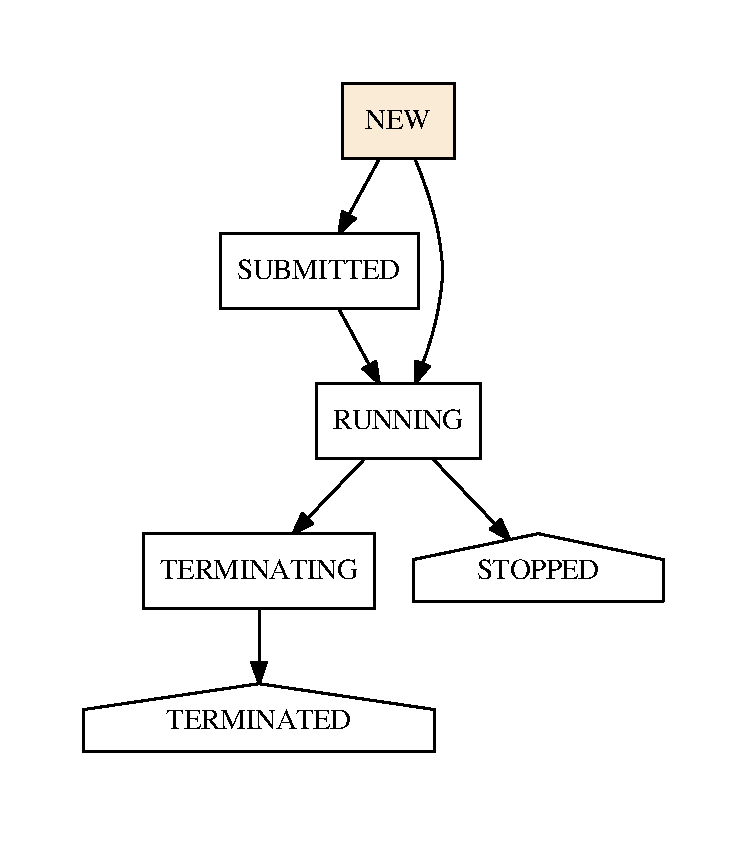
\includegraphics[height=0.7\textheight]{fig/states-NEW}
  \end{column}
  \begin{column}{0.5\textwidth}
    \raggedleft
    \textbf{NEW} is the state of ``just created'' Application objects.

    \+
    The Application has not yet been sent off to a compute
    resource: it only exists locally.
  \end{column}
\end{columns}
\end{frame}


\begin{frame}[fragile]
\frametitle{Application lifecycle: state SUBMITTED}

\begin{columns}[c]
  \begin{column}{0.5\textwidth}
    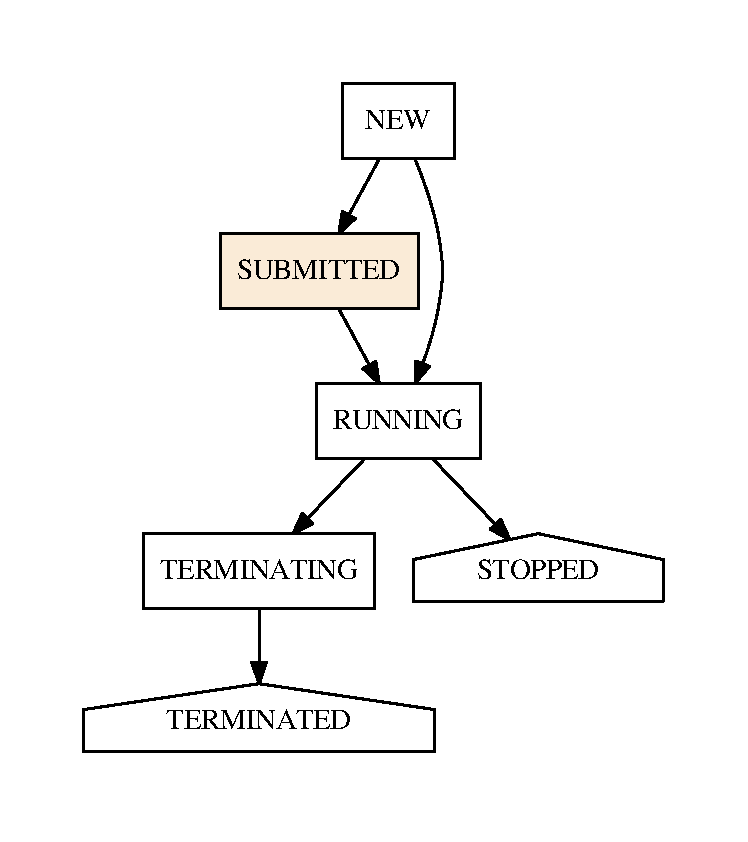
\includegraphics[height=0.7\textheight]{fig/states-SUBMITTED}
  \end{column}
  \begin{column}{0.5\textwidth}
    \raggedleft
    \emph{SUBMITTED} applications have been successfully sent to a
    computational resource.

    \+
    (The transition to \emph{RUNNING} happens automatically, as we
    do not control the remote execution.)
  \end{column}
\end{columns}
\end{frame}


\begin{frame}[fragile]
\frametitle{Application lifecycle: state RUNNING}

\begin{columns}[c]
  \begin{column}{0.5\textwidth}
    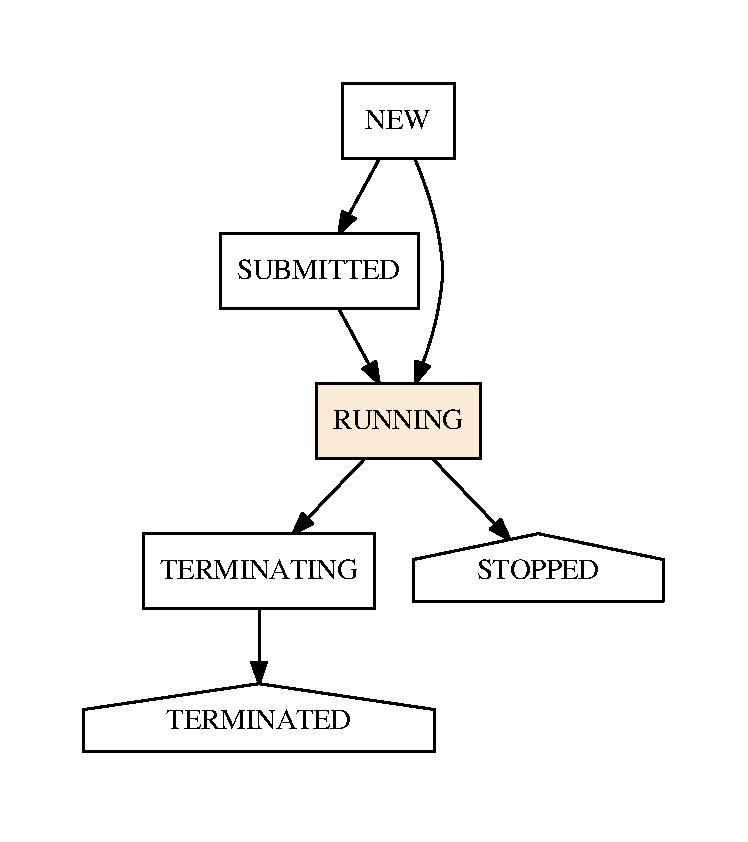
\includegraphics[height=0.7\textheight]{fig/states-RUNNING}
  \end{column}
  \begin{column}{0.5\textwidth}
    \raggedleft
    \emph{RUNNING} state happens when the computational job associated to an
    application starts executing on the computational resource.
  \end{column}
\end{columns}
\end{frame}


\begin{frame}[fragile]
\frametitle{Application lifecycle: state STOPPED}

\begin{columns}[c]
  \begin{column}{0.5\textwidth}
    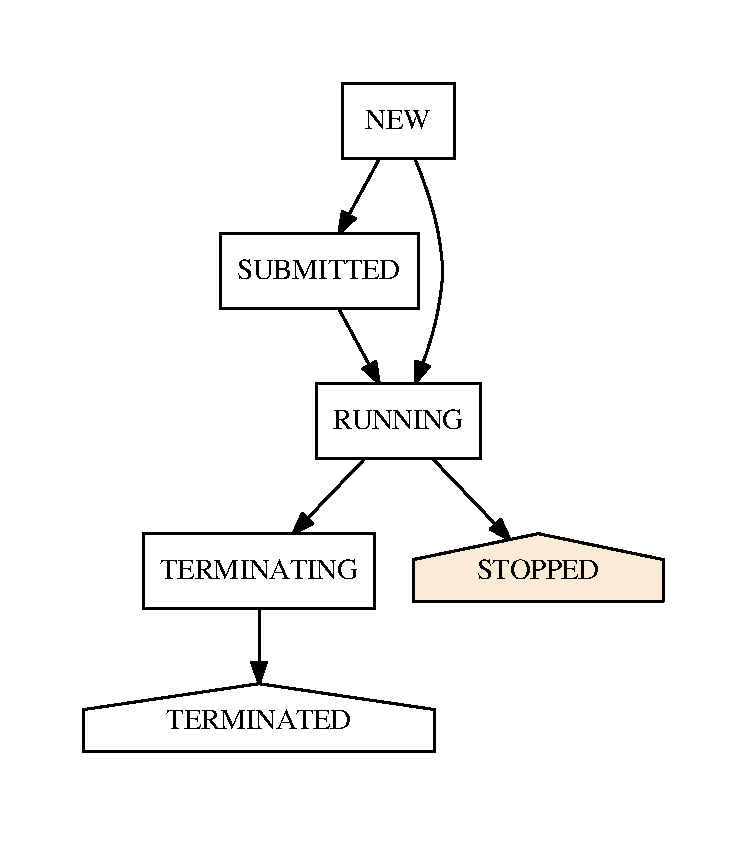
\includegraphics[height=0.7\textheight]{fig/states-STOPPED}
  \end{column}
  \begin{column}{0.5\textwidth}
    \raggedleft
    A task is in \emph{STOPPED} state when its execution has been
    blocked at the remote site and GC3Pie cannot recover
    automatically.

    \+
    User or sysadmin intervention is required for a task to get out
    of \emph{STOPPED} state.
  \end{column}
\end{columns}
\end{frame}


\begin{frame}[fragile]
\frametitle{Application lifecycle: state UNKNOWN}

\begin{columns}[c]
  \begin{column}{0.5\textwidth}
    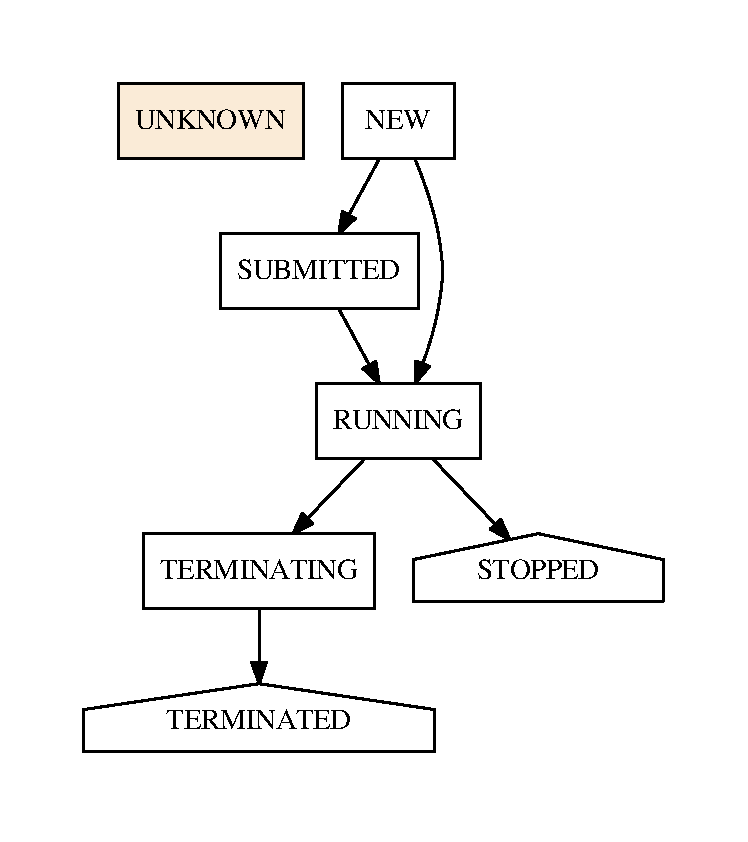
\includegraphics[height=0.7\textheight]{fig/states-UNKNOWN}
  \end{column}
  \begin{column}{0.5\textwidth}
    \raggedleft
    A task is in \emph{UNKNOWN} state when GC3Pie can no
    longer monitor it at the remote site.

    \+
    (As this might be due to network failures, jobs \emph{can} get
    out of \emph{UNKNOWN} automatically.)
  \end{column}
\end{columns}
\end{frame}


\begin{frame}[fragile]
\frametitle{Application lifecycle: state TERMINATING}

\begin{columns}[c]
  \begin{column}{0.5\textwidth}
    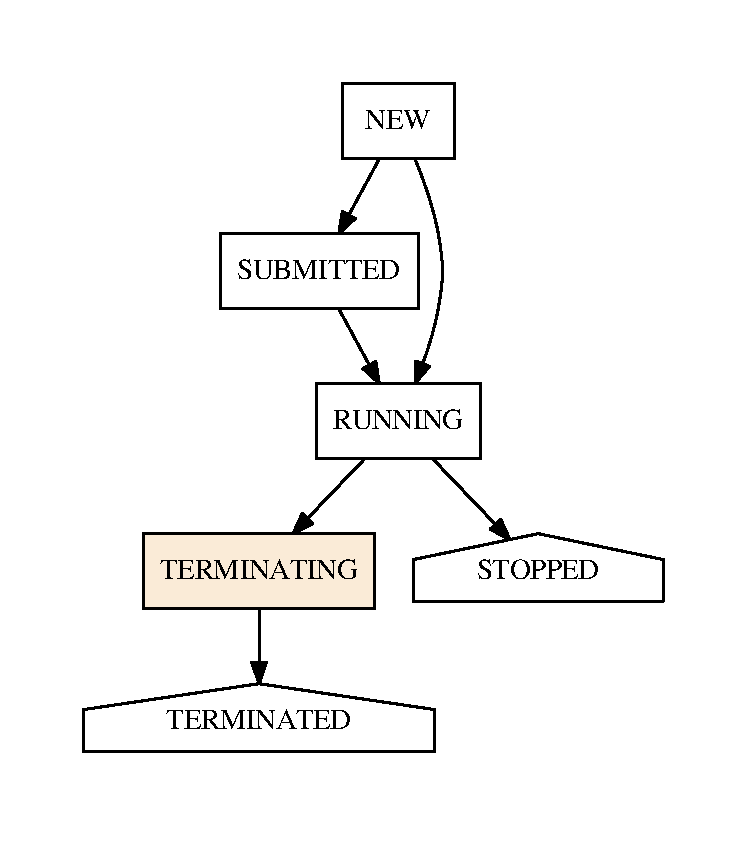
\includegraphics[height=0.7\textheight]{fig/states-TERMINATING}
  \end{column}
  \begin{column}{0.5\textwidth}
    \raggedleft
    \emph{TERMINATING} state when a computational job has finished
    running, for whatever reason.

    \+
    (Transition to \emph{TERMINATED} only happens when \texttt{fetch\_output} is called.)
  \end{column}
\end{columns}
\end{frame}


\begin{frame}[fragile]
\frametitle{Application lifecycle: state TERMINATED}

\begin{columns}[c]
  \begin{column}{0.5\textwidth}
    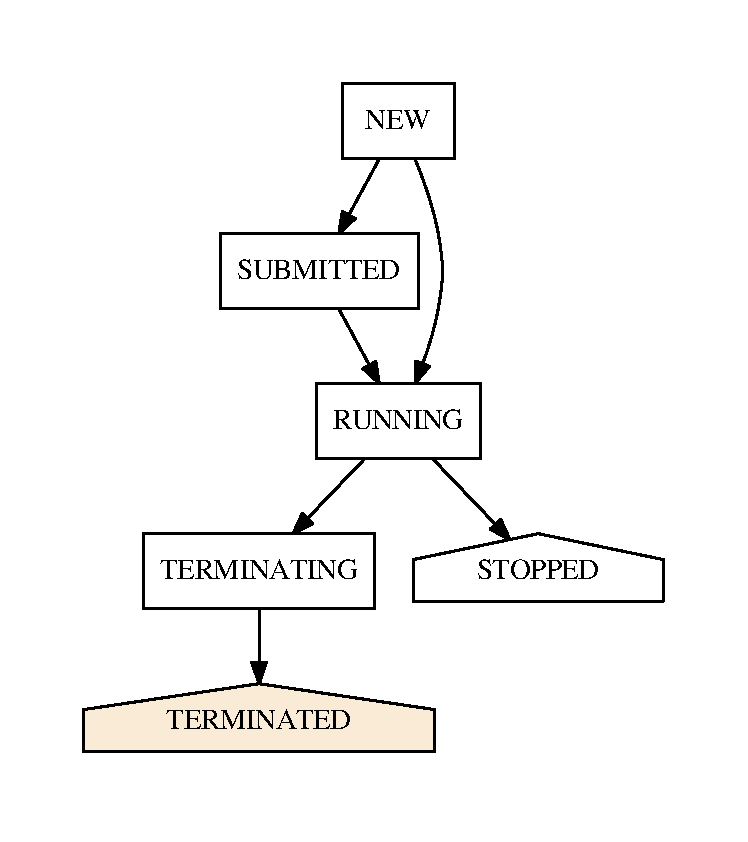
\includegraphics[height=0.7\textheight]{fig/states-TERMINATED}
  \end{column}
  \begin{column}{0.5\textwidth}
    \raggedleft
    A job is \emph{TERMINATED} when its final output has been
    retrieved and is available locally.

    \+
    The exit code of \emph{TERMINATED} jobs can be inspected to
    find out whether the termination was successful or unsuccessful,
    or if the program was forcibly ended.
  \end{column}
\end{columns}
\end{frame}


\section{Post-processing}
\part{Post-processing}

\begin{frame}[fragile]
  \frametitle{Post-processing features, I}

  When the remote computation is done, the \texttt{terminated} method
  of the application instance is called.

  \+
  The path to the output directory is available as
  \lstinline|self.output_dir|; if \texttt{stdout} and \texttt{stderr}
  have been captured, the \textbf{relative} paths to the capture files
  are available as \lstinline|self.stdout| and
  \lstinline|self.stderr|.
\end{frame}


\begin{frame}[fragile]
  \frametitle{Post-processing features, II}

  For example, the following code logs a warning message if the
  standard error output is non-empty:
\begin{python}
class MyApp(Application):
  # ...
  def terminated(self):
    stderr_file = self.output_dir+"/"+self.stderr
    stderr_size = os.stat(stderr_file).st_size
    if stderr_size > 0:
      gc3libs.log.warn(
        "Application %s reported errors!", self)
\end{python}
\end{frame}


\begin{frame}
  \begin{exercise*}[6.A]

    In the \texttt{colorize.py} script from Exercise 4.A, modify the
    \texttt{ColorizeApp} application to move the output picture file
    into directory \texttt{/home/ubuntu/pictures}.  You might need to
    store the output file name to have it available when the
    application has terminated running.

    \+
    (You might want to check out
    \url{http://stackoverflow.com/a/8858026/459543} if you're unsure
    how to move/rename a file with Python.)
  \end{exercise*}
\end{frame}


\section{Termination status}
\part{Termination status}

\begin{frame}[fragile]
  \frametitle{A successful run or not?}

  There's a \emph{single TERMINATED state}, whatever the task outcome.
  You have to inspect the ``return code'' to determine the
  cause of ``task death''.

  \+
  Attribute \lstinline|.execution.returncode| provides a numeric termination
  status (with the same format and meaning as the POSIX termination
  status).

  \+
  The termination status combines two fields: the ``termination
  signal'' and the ``exit code''.

\end{frame}

\begin{frame}[fragile]
  \frametitle{Termination signal, I}

  The \texttt{.execution.signal} instance attribute is non-zero if
  the program was killed by a signal (e.g., memory error / segmentation fault).

  \+
  The \texttt{.execution.signal} instance attribute is zero only if
  the program run until termination. (\textbf{Beware!} This does not
  mean that it run \emph{correctly}: just that it halted by itself.)
\end{frame}


\begin{frame}[fragile]
  \frametitle{Termination signal, II}

  Read
  \href{http://man7.org/linux/man-pages/man7/signal.7.html}{\texttt{man
      7 signal}} for a list of OS signals and their numeric values.

  \+
  {\bfseries Note that GC3Pie overloads some signal codes (unused
    by the OS) to represent its own specific errors.}

  \+
  For instance, if program \texttt{app} was cancelled by the user,
  \texttt{.execution.signal} will take the value 121:
\begin{python}
>>> print(app.execution.signal)
121
\end{python}

\begin{references}
  \tiny\url{https://github.com/uzh/gc3pie/blob/master/gc3libs/__init__.py#L1579}
\end{references}
\end{frame}


\begin{frame}[fragile]
  \frametitle{Exit code}

  The \texttt{.execution.exitcode} instance attribute holds the
  numeric exitcode of the executed command, or \texttt{None} if the
  command has not finished running yet.

  \+
  {\bfseries Note that the \texttt{.execution.exitcode} is guaranteed
    to have a valid value only if the \texttt{.execution.signal}
    attribute has the value 0.}

  \+
  The \texttt{.execution.exitcode} is the same exitcode that you
  would see when running a command directly in the terminal shell. (By
  convention, code 0 is successful termination, every other value
  indicates an error.)
\end{frame}


\begin{frame}
  \begin{exercise*}[6.B]

    Modify the grayscaling script \texttt{ex2c} (or the code it
    depends upon) so that, when a \texttt{GrayscaleApp} task has
    terminated execution, it prints:
    \begin{itemize}
    \item whether the program has been killed by a signal, and the signal number;
    \item whether the program has terminated by exiting, and the exit code.
    \end{itemize}
  \end{exercise*}
\end{frame}


\begin{frame}
  \begin{exercise*}[6.B+] \emph{(Bonus points)} Abstract the verbose
    \texttt{terminated} method from exercise 6.B into an application
    class \texttt{TermStatusApp}.

    \+
    Use Python class inheritance to add the \texttt{TermStatusApp}
    functionality into \texttt{GrayscaleApp}.
  \end{exercise*}
\end{frame}


\begin{frame}[fragile]\small
  \frametitle{Application-specific configuration}

  Application classes may be tagged so that parts of the configuration
  file can be overridden just for them.

  \+
  Suppose you tag the \texttt{GrayscaleApp} class by giving it this name:
\begin{python}
  class GrayscaleApp(Application):
    application_name = 'grayscale'
    # ~\itshape [\ldots]~
\end{python}
  then you can provide a specific VM image just for
  ``\texttt{grayscale}'' applications:
  \begin{stdout}
  # in the GC3Pie config file:
  [resource/sciencecloud]
  # ~\itshape [\ldots]~
  image_id=2b227d15-8f6a-42b0-b744-ede52ebe59f7
  grayscale_image_id=0cca5346-ca12-4cb4-8007-8875c10cce02
  \end{stdout}

  \+ Other configuration items that can be specialized are:
  \lstinline|instance_type|, \lstinline|user_data| (cloud),
  and \lstinline|prolog_file|, \lstinline|epilog_file|
  (batch-systems).
\end{frame}


\begin{frame}[fragile]
  \begin{exercise*}[6.C] \emph{(Difficult)} \small

    MATLAB has the annoying habit of exiting with code 0 even when some error occurred.

    \+
    Write a \texttt{MatlabApp} application, which:
    \begin{itemize}
    \item is constructed by giving the path to a MATLAB `\texttt{.m}'
      script file, like this: \texttt{app = MatlabApp("\href{https://github.com/uzh/gc3pie/blob/master/docs/programmers/tutorials/workflows/downloads/ra.m}{ra.m}")};
    \item Runs the following command:
\begin{semiverbatim}
matlab -nodesktop -nojvm \emph{file.m}
\end{semiverbatim}
      where \emph{file.m} is the file given to the
      \texttt{MatlabApp()} constructor.
    \item captures the standard error output (\texttt{stderr}) of the
      MATLAB script and, if the string ``\texttt{Out of memory.}''
      occurs in it, sets the application exitcode to 11.
    \end{itemize}

    Verify that it works by running MATLAB script
    \href{https://github.com/uzh/gc3pie/blob/master/docs/programmers/tutorials/workflows/downloads/ra.m}{\texttt{ra.m}}
    many times over.  The script initializes a array of random size:
    for some values, the size exceeds the amount of available memory.
  \end{exercise*}
\end{frame}


% \begin{frame}[fragile]
%   \frametitle{Global post-processing}
%   To add some code which will be executed \emph{just before the script
%     exits,} add a \lstinline|after_main_loop| method:

%   \begin{python}
% def after_main_loop(self):
%   model_names = {}
%   for app in ~\HL{self.session.tasks.values()}~:
%     if app.execution.state != Run.State.TERMINATED:
%       return
%     if app.model_name in model_names:
%         model_names[app.model_name] += 1
%     else:
%         model_names[app.model_name] = 1
%   \end{python}

%   \begin{itemize}
%   \item \lstinline|self.session.tasks| is a map
%     \lstinline|JobID|~$\Rightarrow$~\lstinline|Application| object
%   \item \lstinline|self.session.tasks.values()| thus contains a list
%     of all the \textbf{Application}s created by the \lstinline|new_tasks|
%   \end{itemize}
% \end{frame}


\begin{frame}
  \frametitle{Global post-processing}
Further options for customizing a session-based script:
\begin{description}
\item [\texttt{before\_main\_loop(self)}] to execute some code
  \emph{before} the submission of the jobs.
\item [\texttt{after\_main\_loop(self)}] to execute some code
  \emph{after} the main loop. A list of all Application objects is
  available in the \lstinline|self.session.tasks.values()| list.
\end{description}
\end{frame}


\end{document}

%%% Local Variables:
%%% mode: latex
%%% TeX-master: t
%%% End:
